\documentclass[12pt]{article}
\usepackage[utf8]{inputenc}
\usepackage[T1]{fontenc}
\usepackage{amsmath}
\usepackage{amsfonts}
\usepackage{amssymb}
\usepackage[version=4]{mhchem}
\usepackage{stmaryrd}
\usepackage{graphicx}
\usepackage[export]{adjustbox}
\graphicspath{ {./images/} }

\usepackage{listings} % Required for insertion of code
\usepackage{xcolor} % Required for custom colors

% Define custom colors
\definecolor{codegreen}{rgb}{0,0.6,0}
\definecolor{codegray}{rgb}{0.5,0.5,0.5}
\definecolor{codepurple}{rgb}{0.58,0,0.82}
\definecolor{backcolour}{rgb}{0.95,0.95,0.92}

% Setup the style for code listings
\lstdefinestyle{mystyle}{
    backgroundcolor=\color{backcolour},   
    commentstyle=\color{codegreen},
    keywordstyle=\color{magenta},
    numberstyle=\tiny\color{codegray},
    stringstyle=\color{codepurple},
    basicstyle=\ttfamily\footnotesize,
    breakatwhitespace=false,         
    breaklines=true,                 
    captionpos=b,                    
    keepspaces=true,                 
    numbers=left,                    
    numbersep=5pt,                  
    showspaces=false,                
    showstringspaces=false,
    showtabs=false,                  
    tabsize=2
}

% Activate the style
\lstset{style=mystyle}


\title{Ch14 Winter term 2024 \\
 Problem set 5 \\
 due May 30, 2024 }

\author{}
\date{}


\begin{document}
\maketitle
\section{}
An anaerobic denitrification process termed anammox (for anaerobic ammonia oxidation) was identified in microorganisms from the Black Sea. This process involves the net reaction between one molecule of nitrite $\left(\mathrm{NO}_{2}^{-}\right)$ and one molecule of ammonia $\left(\mathrm{NH}_{3}\right)$ to form one molecule of $\mathrm{N}_{2}$. Eq. A

$$
\mathrm{NO}_{2}^{-}+\mathrm{NH}_{3} \quad \rightarrow \quad \mathrm{N}_{2} \quad \text { (unbalanced!!!!) }
$$
\subsection{}

Write a balanced equation for the reduction half reaction for the anammox process.
\subsubsection{Answer}
We started by assigning oxidation states to the individual atoms:
\begin{equation}
\begin{array}{l}
\text { N in } \mathrm{NO}_{2}^{-} \text { is }+3 \\
\text { N in } \mathrm{NH}_{3} \text { is }-3
\end{array}
\end{equation}
since the oxidation states of oxygen and hydrogen are -2 and +1, respectively.
So we identify the unbalanced reduction half reaction as
\begin{equation}
\mathrm{NO}_{2}^{-} \rightarrow \mathrm{N}_{2}
\end{equation}
The next thing we do is to balance the number of elements 
\begin{equation}
2 \mathrm{NO}_{2}^{-} \rightarrow \mathrm{N}_{2}
\end{equation}
Next, we want to balance the number of oxygen atoms by adding two water molecules to the right-hand side of the equation
\begin{equation}
2 \mathrm{NO}_{2}^{-} \rightarrow \mathrm{N}_{2}+2 \mathrm{H}_{2} \mathrm{O}
\end{equation}
Finally, we need to balance the number of hydrogens by adding four protons to the left-hand side of the equation
\begin{equation}
2 \mathrm{NO}_{2}^{-}+4 \mathrm{H}^{+} \rightarrow \mathrm{N}_{2}+2 \mathrm{H}_{2} \mathrm{O}
\end{equation}
Finally, we balance the charge by adding 2 electrons to the left side of the equation:
\begin{equation}
2 \mathrm{NO}_{2}^{-}+4 \mathrm{H}^{+}+2 \mathrm{e}^{-} \rightarrow \mathrm{N}_{2}+2 \mathrm{H}_{2} \mathrm{O}
\end{equation}
\subsection{}

Write a balanced equation for the oxidation half reaction for the anammox process.
\subsubsection{Answer}
We know that the oxidation half reaction is:
\begin{equation}
\mathrm{NH}_{3} \rightarrow \mathrm{N}_{2}
\end{equation}
The next thing we do is to balance the number of nitrogen atoms:
\begin{equation}
2 \mathrm{NH}_{3} \rightarrow \mathrm{N}_{2}
\end{equation}
There are no oxygen atoms to balance, so we just add six protons to the right-hand side:
\begin{equation}
2 \mathrm{NH}_{3} \rightarrow \mathrm{N}_{2}+6 \mathrm{H}^{+}
\end{equation}
Finally, we balance the charge by adding 6 electrons to the right-hand side:
\begin{equation}
2 \mathrm{NH}_{3} \rightarrow \mathrm{N}_{2}+6 \mathrm{H}^{+}+6 \mathrm{e}^{-}
\end{equation}
\subsection{}

Write a balanced equation for the overall anammox process.
\subsubsection{Answer}
The reduction half reaction is:
\begin{equation}
2 \mathrm{NO}_{2}^{-}+4 \mathrm{H}^{+}+2 \mathrm{e}^{-} \rightarrow \mathrm{N}_{2}+2 \mathrm{H}_{2} \mathrm{O}
\end{equation}
The oxidation half reaction is:
\begin{equation}
2 \mathrm{NH}_{3} \rightarrow \mathrm{N}_{2}+6 \mathrm{H}^{+}+6 \mathrm{e}^{-}
\end{equation}
We can multiply the reduction half reaction by a factor of 3:
\begin{equation}
6 \mathrm{NO}_{2}^{-}+12 \mathrm{H}^{+}+6 \mathrm{e}^{-} \rightarrow 3 \mathrm{N}_{2}+6 \mathrm{H}_{2} \mathrm{O}
\end{equation}
Adding the two equations together, we get the overall anammox process:
\begin{equation}
6 \mathrm{NO}_{2}^{-}+6 \mathrm{H}^{+}+2 \mathrm{NH}_{3} \rightarrow 4 \mathrm{N}_{2}+6 \mathrm{H}_{2} \mathrm{O}
\end{equation}


\section{}
\subsection{}

Calculate $\mathrm{E}^{\circ}$ and $\mathrm{E}^{\circ \prime}$ for the reduction of $\mathrm{CO}_{2}$ to $\mathrm{CH}_{4}$:

$$
\mathrm{CO}_{2}(\mathrm{~g})+8 \mathrm{H}^{+}+8 \mathrm{e}^{-} \leftrightarrow \mathrm{CH}_{4}(\mathrm{~g})+2 \mathrm{H}_{2} \mathrm{O}
$$

from the following half-cell reactions:

$$
\begin{array}{ll}
\mathrm{CO}_{2}(\mathrm{~g})+2 \mathrm{H}^{+}+2 \mathrm{e}^{-} \leftrightarrow \mathrm{HCOOH} & \mathrm{E}^{\circ}=-0.199 \mathrm{~V} \\
\mathrm{HCOOH}+2 \mathrm{H}^{+}+2 \mathrm{e}^{-} \leftrightarrow \mathrm{HCHO}+\mathrm{H}_{2} \mathrm{O} & \mathrm{E}^{\circ}=0.034 \mathrm{~V} \\
\mathrm{HCHO}+2 \mathrm{H}^{+}+2 \mathrm{e}^{-} \leftrightarrow \mathrm{CH}_{3} \mathrm{OH} & \mathrm{E}^{\circ}=0.232 \mathrm{~V} \\
\mathrm{CH}_{3} \mathrm{OH}+2 \mathrm{H}^{+}+2 \mathrm{e}^{-} \leftrightarrow \mathrm{CH}_{4}(\mathrm{~g})+\mathrm{H}_{2} \mathrm{O} & \mathrm{E}^{\circ}=0.588 \mathrm{~V}
\end{array}
$$
\subsubsection{Answer}
If we add all of the half-cell reactions together, we get the full reduction that we are considering, so all that is left is that we need to add all of the standard reduction potentials together to get the standard reduction potential for the full reaction:
\begin{equation}
\begin{aligned}
\mathrm{E}^{\circ} &=\sum \mathrm{E}^{\circ} \\
&=-0.199+0.034+0.232+0.588 \\
&=0.655 \mathrm{~V}
\end{aligned}
\end{equation}
The Nernst equation is:
\begin{equation}
\mathrm{E}^{\circ \prime}=\mathrm{E}^{\circ}-\frac{0.0592}{8} \log \left(\frac{1}{K_{\mathrm{eq}}}\right)
\end{equation}
where $K_{\mathrm{eq}}$ is the equilibrium constant for the reaction. We can calculate $K_{\mathrm{eq}}$ from the standard reduction potential:
\begin{equation}
\begin{aligned}
\Delta G^{\circ} &=-n F \Delta E^{\circ} \\
&=-8 \times 96485 \times 0.655 \\
&=-5.06 \times 10^{5} \mathrm{~J} / \mathrm{mol}
\end{aligned}
\end{equation}
\begin{equation}
\begin{aligned}
K_{\mathrm{eq}} &=\exp \left(-\frac{\Delta G^{\circ}}{R T}\right) \\
&=\exp \left(-\frac{-5.06 \times 10^{5}}{8.314 \times 298}\right) \\
&=4.20 \times 10^{88}
\end{aligned}
\end{equation}
Finally, we can calculate the Nernst potential:
\begin{equation}
\begin{aligned}
\mathrm{E}^{\circ \prime} &=0.655-\frac{0.0592}{8} \log \left(\frac{1}{4.20 \times 10^{88}}\right) \\
&=1.31 \mathrm{~V}
\end{aligned}
\end{equation}
\subsection{}

From these results, calculate $\Delta \mathrm{G}^{\circ}($ at $\mathrm{pH}=0)$ and $\Delta \mathrm{G}^{\circ}{ }^{\circ}(\mathrm{pH}=7)$ for the reduction of one mole of $\mathrm{CO}_{2}$ to $\mathrm{CH}_{4}$ coupled to the oxidation of $\mathrm{H}_{2}$. (Hint: $\Delta \mathrm{G}^{\circ 1} \sim-127 \mathrm{~kJ} / \mathrm{mole}$ - but show your work)
\subsubsection{Answer}
The standard Gibbs free energy change $\Delta G^{\circ}$ can be calculated from the standard reduction potential $\mathrm{E}^{\circ}$ using the formula:
\begin{equation}
\Delta G^{\circ}=-n F \Delta E^{\circ}
\end{equation}
We can calculate $\Delta G^{\circ}$ at $\mathrm{pH}=0$ using the standard reduction potential $\mathrm{E}^{\circ}$:
\begin{equation}
\begin{aligned}
\Delta G^{\circ}(\mathrm{pH}=0) &=-8 \times 96485 \times 0.655 \\
&=-5.06 \times 10^{5} \mathrm{~J} / \mathrm{mol} \\
&=-506 \mathrm{~kJ} / \mathrm{mol}
\end{aligned}
\end{equation}
To calculate $\Delta G^{\circ}$ at $\mathrm{pH}=7$, we need to consider the effect of the pH on the standard reduction potential. The Nernst equation is:
\begin{equation}
\mathrm{E}^{\circ \prime}=\mathrm{E}^{\circ}-\frac{0.0592}{8} \log \left(Q\right)
\end{equation}
where $Q$ is the reaction quotient. That corresponding equation for a change in pH is a modified Nernst equation:
\begin{equation}
\mathrm{E}^{\circ \prime}=\mathrm{E}^{\circ}-\frac{0.0592}{8} \log \left([\text{products}]/[\text{reactants}]\right) - \frac{0.0592 h}{8} \text{pH}
\end{equation}
where $h$ is the number of protons involved in the reaction. But since we found that the equilibrium constant is very large, we can neglect the middle term:
\begin{equation}
E^{\circ \prime}=E^{\circ}-\frac{0.0592\times 8}{8}\times 7 = 0.655-0.0592\times 7 = 0.655-0.4144 = 0.2406 \mathrm{~V}
\end{equation}
Now come we can calculate the standard Gibbs free energy change $\Delta G^{\circ \prime}$ at $\mathrm{pH}=7$:
\begin{equation}
\Delta G^{\circ \prime} = -n F \Delta E^{\circ \prime} = -8 \times 96485 \times 0.2406 = -186 \mathrm{~kJ} / \mathrm{mol}
\end{equation}




\subsection{}
Write a balanced equation for the half-cell reaction corresponding to the reduction of two moles of $\mathrm{CO}_{2}$ to form one mole of acetic acid $\left(\mathrm{CH}_{3} \mathrm{CO}_{2} \mathrm{H}\right)$.
\subsubsection{Answer}
The given equation has two moles of carbon dioxide on the left and one mole of acetic acid on the right:
\begin{equation}
2 \mathrm{CO}_{2}\rightarrow \mathrm{CH}_{3} \mathrm{CO}_{2} \mathrm{H}
\end{equation}
The carbons are balanced, so the next thing we need to do is to balance the number of oxygen atoms by adding 2 water molecules to the right side:
\begin{equation}
2 \mathrm{CO}_{2}\rightarrow \mathrm{CH}_{3} \mathrm{CO}_{2} \mathrm{H}+2 \mathrm{H}_{2} \mathrm{O}
\end{equation}
Finally, we need to balance the number of hydrogens by adding 8 protons to the left side:
\begin{equation}
2 \mathrm{CO}_{2}+8 \mathrm{H}^{+}\rightarrow \mathrm{CH}_{3} \mathrm{CO}_{2} \mathrm{H}+2 \mathrm{H}_{2} \mathrm{O}
\end{equation}
Finally, we need to balance the charge by adding 8 electrons to the left side:
\begin{equation}
2 \mathrm{CO}_{2}+8 \mathrm{H}^{+}+8 \mathrm{e}^{-}\rightarrow \mathrm{CH}_{3} \mathrm{CO}_{2} \mathrm{H}+2 \mathrm{H}_{2} \mathrm{O}
\end{equation}

\subsection{}
If $\Delta \mathrm{G}^{\circ}=-37 \mathrm{~kJ} / \mathrm{mole}$ for disproportionation of acetic acid to methane and $\mathrm{CO}_{2}$ :

$$
\mathrm{CH}_{3} \mathrm{CO}_{2} \mathrm{H} \leftrightarrow \mathrm{CH}_{4}+\mathrm{CO}_{2}
$$

calculate $\mathrm{E}^{\circ+}$ for the reduction of two moles of $\mathrm{CO}_{2}$ to one mole of acetic acid.
\subsubsection{Answer}
If we flip the given reaction around we get:
\begin{equation}
\mathrm{CH}_{4}+\mathrm{CO}_{2}\rightarrow \mathrm{CH}_{3} \mathrm{CO}_{2} \mathrm{H}
\end{equation}
and this will have the opposite free energy change, now of $37 \mathrm{~kJ} / \mathrm{mol}$. If we add the initial reaction of carbon dioxide to methane that has already been balanced to this, we get the overall reaction:
\begin{equation}
2 \mathrm{CO}_{2}+8 \mathrm{H}^{+}+8 \mathrm{e}^{-} \rightarrow \mathrm{CH}_{3} \mathrm{CO}_{2} \mathrm{H} +2 \mathrm{H}_{2} \mathrm{O}
\end{equation}
Adding the $\Delta G^{\circ}$ values together, we get:
\begin{equation}
37-186 = -149 \mathrm{~kJ} / \mathrm{mol}
\end{equation}



\section{}
Flavins can exist in three oxidation states, fully oxidized (ox), semi-quinone (sq) and the fully reduced hydroquinone ( $\mathrm{hq}$ ) that are related by the following scheme:

$$
\mathrm{ox}+\mathrm{e}^{-} \stackrel{E_{1}{ }^{\circ \prime}}{\longleftrightarrow} \mathrm{sq}+\mathrm{e}^{-} \stackrel{E_{2}{ }^{\circ \prime}}{\longleftrightarrow} \mathrm{hq}
$$

At equilibrium, a solution of flavin will equilibrate between the three states according to the disproportionation reaction with equilibrium constant $\mathrm{K}_{\mathrm{dp}}$:

$$
2 \mathrm{sq} \leftrightarrow \mathrm{ox}+\mathrm{hq}
$$

For a flavin bound to a particular protein (designated FLD), $\mathrm{E}_{1}^{\circ \prime}$ and $\mathrm{E}_{2}^{\circ}$ are $-0.200 \mathrm{~V}$ and -0.450 $\mathrm{V}$, respectively, while the corresponding values for the free flavin (designated FMN) are -0.300 $\mathrm{V}$ and $-0.125 \mathrm{~V}$, respectively.
\subsection{}
From these reduction potentials, calculate the values of the equilibrium constant $\mathrm{K}_{\mathrm{dp}}$ for the disproportionation reactions of FLD and FMN.
\subsubsection{Answer}
We have two given reactions that would be represented by:
\begin{equation}
\begin{array}{l}
\mathrm{ox}+\mathrm{e}^{-} \rightarrow \mathrm{sq} \\
\mathrm{sq}+\mathrm{e}^{-} \rightarrow \mathrm{hq}
\end{array}
\end{equation}
If we flip the first one around, then adding the two half-reactions would give the desired disproportionation reaction. So we can use the second reduction potential and add the negation of the first potential to represent the potential for the overall disproportionation reaction. We can use the obtained reduction potential to calculate the free energy change for the disproportionation reaction and thus also the equilibrium constant. Note that we want to do this process for the two separate cases of FLD and FMN. The equilibrium constant for the disproportionation reaction of FLD is $5.91 \times 10^{-5}$, and for FMN it is $9.11 \times 10^{2}$.
% Inline Python code in the document
\begin{lstlisting}[language=Python]
import sympy as sp

# Constants
F = 96485  # Faraday's constant in C/mol
R = 8.314  # Gas constant in J/(mol*K)
T = 298  # Temperature in K

# Reduction potentials for FLD and FMN
E1_FLD = -0.2 # Volts
E2_FLD = -0.45 # Volts

E1_FMN = -0.3 # Volts
E2_FMN = -0.125 # Volts

# Calculate E_dp for FLD
E_dp_FLD = E2_FLD - E1_FLD

# Calculate free energy change for FLD disproportionation reaction
delta_G_dp_FLD = -1 * F * E_dp_FLD

# Calculate K_dp for FLD
K_dp_FLD = sp.exp(-delta_G_dp_FLD / (R * T))

# Calculate E_dp for FMN
E_dp_FMN = E2_FMN - E1_FMN

# Calculate free energy change for FMN disproportionation reaction
delta_G_dp_FMN = -1 * F * E_dp_FMN

# Calculate K_dp for FMN
K_dp_FMN = sp.exp(-delta_G_dp_FMN / (R * T))

# Display the results
K_dp_FLD.evalf(), K_dp_FMN.evalf()

\end{lstlisting}
\subsection{}
A 1 M FLD solution, initially prepared in the sq state, is allowed to reach equilibrium. What are the concentrations of the ox, sq and hq forms at equilibrium? (note: the $1 \mathrm{M}$ concentration is unrealistic, but it simplifies the calculation).\\

If the same experiment is repeated with a $1 \mathrm{M}$ FMN solution, initially prepared in the sq state, what are the equilibrium concentrations of these three forms?
\subsubsection{Answer}
The definition of the equilibrium constant is given by:
\begin{equation}
K_{\text {dp }}=\frac{[\text {ox }][\text {hq }]}{[\text {sq }]^{2}}
\end{equation}
We know the equilibrium constant and that the initial concentration of sq is 1 M. Therefore, the equilibrium concentration of ox and hq can be given the variable $x$ and so the europium concentration of sq is $1-2x$. We can substitute these values into the equilibrium constant equation and solve for $x$ to get the equilibrium concentrations of the three forms. The concentrations of sq, ox, and hq at equilibrium for FLD are $0.985, 0.00757,$ and $0.00757$ M, respectively. For FMN, the concentrations are $0.0163, 0.492,$ and $0.492$ M, respectively.
% Inline Python code in the document
\begin{lstlisting}[language=Python]
import sympy as sp

# Constants from the previous calculations
K_dp_FLD = 5.91e-5
K_dp_FMN = 9.11e2
K_dp = {'FLD': K_dp_FLD, 'FMN': K_dp_FMN}

# Define the variable for change in concentration
x = sp.symbols('x')

# Initial concentration of sq
sq_initial = 1  # 1 M

# Equilibrium concentrations
sq_eq = sq_initial - 2*x
ox_eq = x
hq_eq = x

# Loop over the two cases to determine the equilibrium concentrations of the three species in each case
for case in ['FLD', 'FMN']:
    # Calculate the equilibrium constant for the disproportionation reaction
    K = K_dp[case]

    # Define the expression for the equilibrium constant
    eq = K - (hq_eq * ox_eq / sq_eq**2)

    # Solve the equation for x
    x_values = sp.solve(eq, x)

    # Filter for realistic solutions (0 <= x <= 0.5)
    real_solutions = [sol for sol in x_values if sol.is_real and 0 <= sol <= 0.5]
    
    if real_solutions:
        x_value = real_solutions[0]
        
        # Calculate the equilibrium concentrations
        sq_eq_value = sq_eq.subs(x, x_value)
        ox_eq_value = ox_eq.subs(x, x_value)
        hq_eq_value = hq_eq.subs(x, x_value)

        # Display the results
        print(f"Case {case}:")
        print(f"[sq]_eq = {sq_eq_value}")
        print(f"[ox]_eq = {ox_eq_value}")
        print(f"[hq]_eq = {hq_eq_value}")

\end{lstlisting}

\section{}
Calculate the solubility product $\mathrm{K}_{\mathrm{sp}}$ at $298 \mathrm{~K}$ for the reaction:

$$
\mathrm{AgBr}(\mathrm{s}) \leftrightarrow \mathrm{Ag}^{+}+\mathrm{Br}^{-}
$$

from the half-cell reactions:

$$
\begin{array}{ll}
\mathrm{Ag}^{+}+\mathrm{e}^{-} \leftrightarrow \mathrm{Ag}(\mathrm{s}) & \mathrm{E}^{\circ}=+0.799 \mathrm{~V} \\
\left.\mathrm{AgBr}^{\mathrm{s}}\right)+\mathrm{e}^{-} \leftrightarrow \mathrm{Ag}(\mathrm{s})+\mathrm{Br}^{-} & \mathrm{E}^{\circ}=+0.071 \mathrm{~V}
\end{array}
$$
\subsection{Answer}
We want to flip the first half reaction around to get the two half cell reactions:
\begin{equation}
\mathrm{Ag}(\mathrm{s}) \rightarrow \mathrm{Ag}^{+}+\mathrm{e}^{-}
\end{equation}
Now, we can add this half cell reaction to the other one to get the desired one using some fortuitous cancellations:
\begin{equation}
\mathrm{AgBr}(\mathrm{s}) \rightarrow \mathrm{Ag}^{+}+\mathrm{Br}^{-}
\end{equation}
The standard reduction potential for this reaction is the sum of the standard reduction potentials for the two half-cell reactions with the first one flipped around:
\begin{equation}
\begin{aligned}
\mathrm{E}^{\circ} &=-\mathrm{E}_{1}^{\circ}+\mathrm{E}_{2}^{\circ} \\
&=-0.799+0.071 \\
&=-0.728 \mathrm{~V}
\end{aligned}
\end{equation}
Using this, we can compute the free energy change:
\begin{equation}
\begin{aligned}
\Delta G^{\circ} &=-n F \Delta E^{\circ} \\
&=-1 \times 96485 \times -0.728 \\
&=70.3 \mathrm{~kJ} / \mathrm{mol}
\end{aligned}
\end{equation}
The equilibrium constant is:
\begin{equation}
\begin{aligned}
K_{\mathrm{sp}} &=\exp \left(-\frac{\Delta G^{\circ}}{R T}\right) \\
&=\exp \left(-\frac{70.3}{8.314 \times 298}\right) \\
&=1.77 \times 10^{-13}
\end{aligned}
\end{equation}


\section{}
The standard reduction potentials for the $\mathrm{Co}^{3+} / \mathrm{Co}^{2+}$ half cell in the absence and presence of a chelating ligand abbreviated "trtda" with a 4- charge, are:

$$
\begin{array}{ll}
\mathrm{Co}^{3+}+\mathrm{e}^{-} \rightarrow \mathrm{Co}^{2+} & \mathrm{E}_{1}{ }^{\circ}=+1.820 \mathrm{~V} \\
\left.\mathrm{Co} (\text{trtda})\right)^{-}+\mathrm{e}^{-} \rightarrow \mathrm{Co}(\text{trtda})^{2-} & \mathrm{E}_{2}^{\circ}=+0.290 \mathrm{~V}
\end{array}
$$

The relationship between these $E^{\circ}$ values and the association constants for the binding of trtda $^{4-}$ to the oxidized and reduced forms of Co are summarized in the following schematic:\\
(B)

\begin{center}
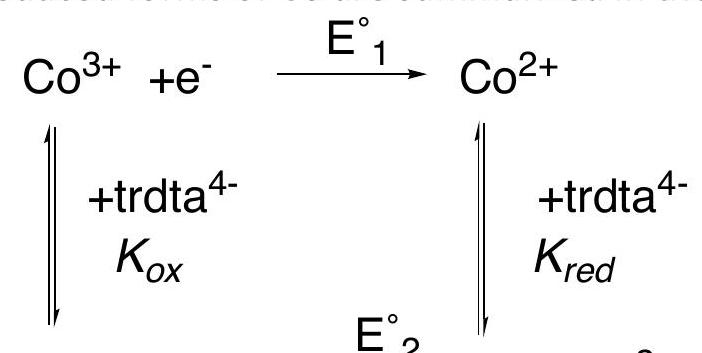
\includegraphics[max width=\textwidth]{2024_05_26_76014722f19b3362a624g-2}
\end{center}

(C)\\
(A)

\begin{center}
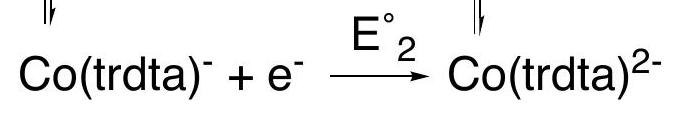
\includegraphics[max width=\textwidth]{2024_05_26_76014722f19b3362a624g-2(1)}
\end{center}

(D)

The association constant, $K_{\text {red }}$, for $\text{trtda}^{4-}$ binding to $\mathrm{Co}^{2+}$ is measured to be $2.45 \times 10^{15}$. From this data, calculate the association constant, $K_{\text{ox}}$, for the binding of $\text{trtda}^{4-}$ to $\mathrm{Co}^{3+}$.
\subsection{Answer}
From the $E^{\circ}_1$ values, we can calculate the free energy change for the first half cell reaction. We do this using the equation:
\begin{equation}
\Delta G^{\circ}_{1}=-n F \Delta E^{\circ}_1
\end{equation}
where $n$ is the number of electrons transferred in the reaction. Then given the value of $K_{\text{red}}$, we can calculate the free energy change for the reduced association:
\begin{equation}
\Delta G^{\circ}_{\text{red}}=-RT \ln K_{\text{red}}
\end{equation}
We also know the reduction potential for the second half reaction, but here we are interested in the free energy change going from products to reactants, so we flip the sign, but use the same equation as before:
\begin{equation}
\Delta G^{\circ}_2=-n F \Delta E^{\circ}_2
\end{equation}
That is, we are really interested in $- \Delta G^{\circ}$ in this case. The free energy change for the entire cycle must be 0:
\begin{equation}
\Delta G^{\circ}_{1}+\Delta G^{\circ}_{\text{red}}-\Delta G^{\circ}_2-\Delta G^{\circ}_{\text{ox}}=0
\end{equation}
We can solve this equation for $\Delta G^{\circ}_{\text{ox}}$ and then use the equation for the free energy change to calculate $K_{\text{ox}}$ as $1.84 \times 10^{41}$.
% Inline Python code in the document
% Inline Python code in the document
\begin{lstlisting}[language=Python]
import sympy as sp

# Constants
F = 96485  # Faraday's constant in C/mol
R = 8.314  # Gas constant in J/(mol*K)
T = 298  # Temperature in K
K_red = 2.45e15  # Association constant for reduced form

# Reduction potentials in V
E1 = 1.820
E2 = 0.290

# Calculate free energy changes
delta_G1 = -1 * F * E1  # Free energy change for the first half-cell reaction
delta_G2 = -1 * F * E2  # Free energy change for the second half-cell reaction with sign flipped
delta_G_red = -R * T * sp.log(K_red)  # Free energy change for the reduced association

# Calculate delta G_ox such that the total free energy change sums to zero
delta_G_ox = delta_G1 + delta_G_red - delta_G2

# Calculate the association constant K_ox
K_ox_corrected = sp.exp(-delta_G_ox / (R * T))

# Convert values to kJ/mol
delta_G1_kj = delta_G1 / 1000
delta_G2_corrected_kj = delta_G2 / 1000
delta_G_red_kj = delta_G_red / 1000
delta_G_ox_corrected_kj = delta_G_ox / 1000

# Display the results
delta_G1_kj, delta_G2_corrected_kj, delta_G_red_kj, delta_G_ox_corrected_kj, K_ox_corrected.evalf()

\end{lstlisting}



\end{document}